\documentclass[tikz]{standalone}

\usepackage{tikz}
\usetikzlibrary{trees}
\usetikzlibrary{shapes}
\usetikzlibrary{positioning}
\usetikzlibrary{arrows.meta}

\tikzset{
    mynode/.style = {circle, ultra thick, draw=black, align=center,fill=yellow!30,font=\ttfamily\bfseries\Large,text=black},
    mynoder/.style = {circle, ultra thick, draw=black, align=center,fill=red!30,font=\ttfamily\bfseries\Large,text=black},
    mynodeb/.style = {circle, ultra thick, draw=black, align=center,fill=blue!30,font=\ttfamily\bfseries\Large,text=black},
    mynodeg/.style = {circle, ultra thick, draw=gray, align=center,fill=gray!05,font=\ttfamily\bfseries\Large,text=gray!20},
    mynodegr/.style = {circle, ultra thick, draw=gray, align=center,fill=gray!05,font=\ttfamily\bfseries\Large,text=red},
    edgen/.style = {-,ultra thick,black},
    edger/.style = {-,ultra thick,red},
    edgeb/.style = {-,ultra thick,blue},
    edgeg/.style = {-,ultra thick,gray},
    edgegd/.style = {-,ultra thick,brown,dashed}, % back
    edgevd/.style = {-,ultra thick,violet,dotted}, % forward
    edgexd/.style = {-,ultra thick,blue,densely dotted}, % traversal
    every picture/.style={/utils/exec={\ttfamily\bfseries}},
    every picture/.style={font issue=\ttfamily\bfseries},
    font issue/.style={execute at begin picture={#1\selectfont}}
}
\usetikzlibrary{shapes.geometric}

\begin{document}

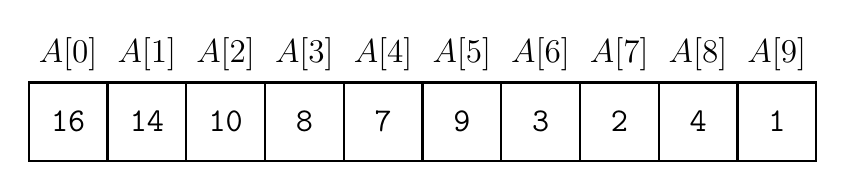
\begin{tikzpicture}[
	thick,
	font=\ttfamily\bfseries\large]
  \node at (0,0) [draw,minimum size=1cm,label={above:$A[0]$}] {16};
  \node at (1,0) [draw,minimum size=1cm,label={above:$A[1]$}] {14};
  \node at (2,0) [draw,minimum size=1cm,label={above:$A[2]$}] {10};
  \node at (3,0) [draw,minimum size=1cm,label={above:$A[3]$}] {8};
  \node at (4,0) [draw,minimum size=1cm,label={above:$A[4]$}] {7};
  \node at (5,0) [draw,minimum size=1cm,label={above:$A[5]$}] {9};
  \node at (6,0) [draw,minimum size=1cm,label={above:$A[6]$}] {3};
  \node at (7,0) [draw,minimum size=1cm,label={above:$A[7]$}] {2};
  \node at (8,0) [draw,minimum size=1cm,label={above:$A[8]$}] {4};
  \node at (9,0) [draw,minimum size=1cm,label={above:$A[9]$}] {1};
\end{tikzpicture}

\end{document}